\chapter{METODOLOGIA}

O trabalho em questão consistirá em uma pesquisa aplicada, com o objetivo de realizar um estudo exploratório fundamentado em material bibliográfico e ensaios de laboratório. Serão utilizados os procedimentos técnicos de pesquisa bibliográfica e experimental. O percurso metodológico adotará o método de abordagem hipotético-dedutivo, complementado pelo método de procedimento monográfico para a sua estruturação e elaboração. No que tange à coleta de dados referentes ao desempenho do microcontrolador, será feito o uso de documentação indireta. A análise e a interpretação desses dados ocorrerão primariamente de forma qualitativa e global, avaliando o comportamento sistêmico da solução.

Inicialmente, será realizada uma revisão sistemática de literatura abordando as áreas centrais que permeiam o projeto: arquiteturas de microcontroladores modernos, sensores e instrumentação, sistemas eletrônicos de tempo real, Sistemas Operacionais Embarcados e as diretrizes do AAS na Indústria 4.0.

Complementarmente à fundamentação teórica, será realizado o estudo das bibliotecas de \textit{software} necessárias para o desenvolvimento do projeto. No escopo da biblioteca que será desenvolvida, destacam-se a avaliação de pilhas compatíveis com o protocolo OPC UA, como a \textit{open62541}, bibliotecas eficientes para serialização e manipulação de arquivos JSON em C/C++, como a \textit{cJSON}, além dos componentes nativos e \textit{drivers} fornecidos pelo \textit{framework} ESP-IDF.

Em seguida, serão desenvolvidos os códigos-fonte da biblioteca proposta neste trabalho. A implementação será focada em arquitetar um núcleo leve capaz de hospedar o AAS dentro das restrições de memória do microcontrolador, integrando as rotinas de comunicação e armazenamento de dados de forma transparente. Adicionalmente, durante o ciclo de desenvolvimento, será realizada a elaboração dos testes unitários necessários para garantir a robustez das funções críticas do sistema, prevenindo falhas de alocação de memória e garantindo a correta serialização dos dados.

Para a validação prática do uso da biblioteca, será desenvolvido um Gêmeo Digital reativo, caracterizado como um AAS do Tipo 2. O planejamento desta fase iniciará com o levantamento das ferramentas e equipamentos de medição, englobando aparelhos como multímetro e osciloscópio para a verificação e calibração dos sinais elétricos.

O \textit{hardware} montado formará a plataforma física do componente, ilustrada na Figura \ref{fig:arquitetura_geral}, enquanto a biblioteca desenvolvida atuará no microcontrolador para disponibilizar os dados na rede.

\clearpage

\begin{figure}[htb]
    \centering
    \caption{Arquitetura geral proposta para a instrumentação do AAS}
    \label{fig:arquitetura_geral}
    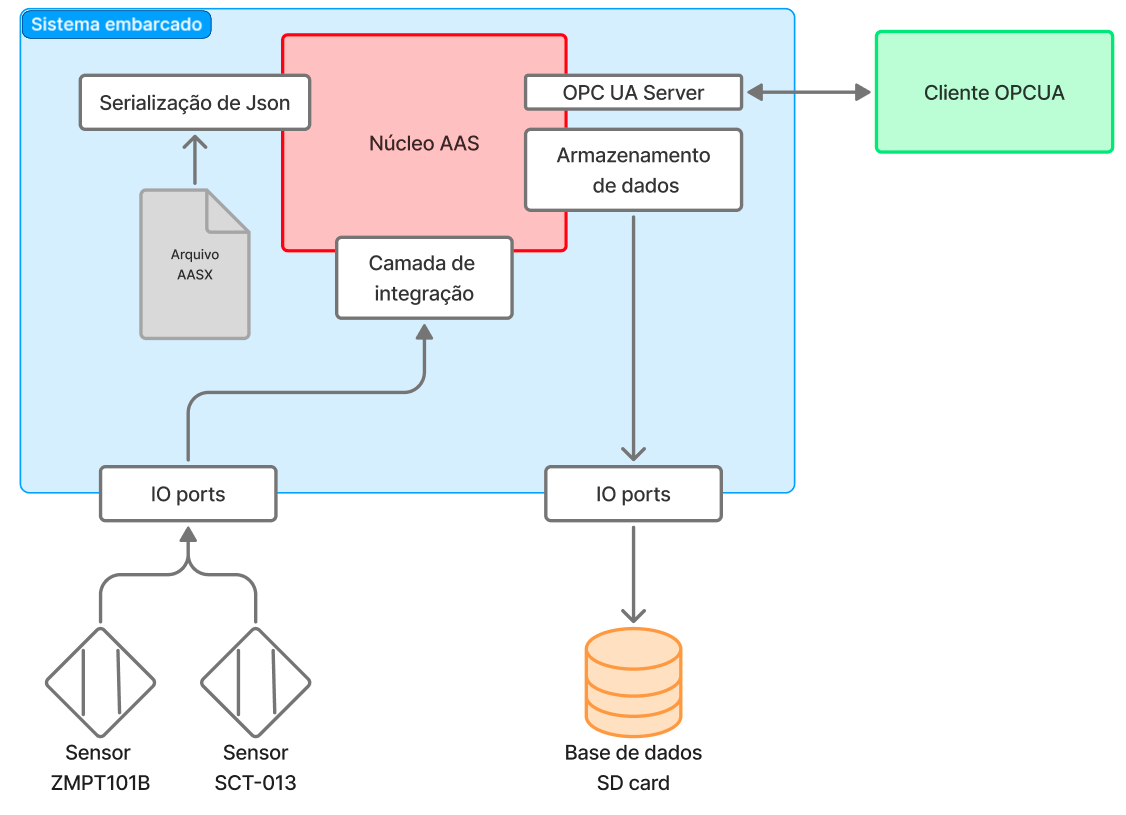
\includegraphics[width=0.60\textwidth]{figuras/arquitetura_geral.png}
    
    \fonte{Elaborado pelo autor.}
\end{figure}

A análise dos resultados será feita por verificação funcional da arquitetura. Serão observados o funcionamento da aquisição de dados, a continuidade da comunicação, a coerência dos registros armazenados e a atualização do gêmeo digital. Com isso, será possível medir e analisar o desempenho do microcontrolador como um AAS embarcado.